\section{Exercise 8}
The inverse for each of the grids were calculated using the $LU$ factorials
of matrix, namely
\begin{equation}
    A^{-1} = U^{-1}L^{-1}
\end{equation}
where the factorials were found using the subroutine discussed in Exercise
6. The following logic was used to find the inverse of matrix $A$: 

\begin{algorithm}[H]
\DontPrintSemicolon
\SetAlgoLined
\KwResult{Calculating $A^{-1}$}
\SetKwInOut{Input}{Input}\SetKwInOut{Output}{Output}
\Input{$A$}
\Output{$A^{-1}$}
\BlankLine
    $[L, U] = \text{LU\_facrorization}(A)$
\BlankLine
    $Linv   = lower\_inverse(L)$\;
    $Uinv   = upper\_inverse(L)$\;
    $Ainv   = Uinv \times Linv $\; 

    \caption{$A^{-1}$ Subroutine}
\end{algorithm}

Where the inverse subroutines use the following logic: \\ 
\begin{algorithm}[H]
\DontPrintSemicolon
\SetAlgoLined
\KwResult{Lower triangular inverse}
\SetKwInOut{Input}{Input}\SetKwInOut{Output}{Output}
\Input{$L$}
\Output{$L^{-1}$}

\BlankLine
    out = identity(M) \;
    \For{j in range(0, M-1)}{ 
        \For{i in range(j,M-1)}{
            c           = mat[i+1,j]\;
            out[i+1,:]  = out[i+1,:]-c*out[j,:]\;
        }
        }
    \caption{$L^{-1}$ Subroutine}
\end{algorithm}
\begin{algorithm}[H]
\DontPrintSemicolon
\SetAlgoLined
\KwResult{Upper triangular inverse}
\SetKwInOut{Input}{Input}\SetKwInOut{Output}{Output}
\Input{$U$}
\Output{$U^{-1}$}

\BlankLine
    out = identity(M) \;
    \For{j in range(M-1, -1, -1)}{ 
        \For{i in range(j, 0, -1)}{
            c           = mat[i-1,j]/mat[j,j]\;
            out[i-1,:]  = out[i-1,:]-c*out[j,:]\;
    }
    out[j,:] = out[j,:]/mat[j,j]
    }
    \caption{$U^{-1}$ Subroutine}
\end{algorithm}

Using the above we get the following result shown in
Fig.~(\ref{fig:inverse-study}), where we can see once again the benefit in
using the pre-compiled optimized code. Lastly, the full inverse code is
provided in the Appendix.
\begin{figure}[H]
    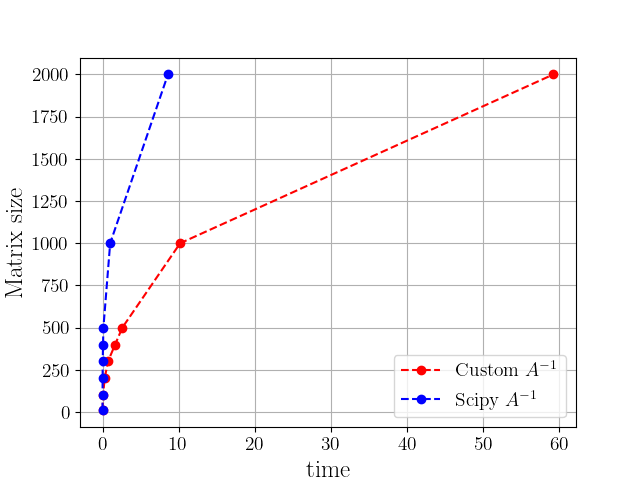
\includegraphics[height=3.0in]{media/exercise-8.png}
    \caption{Performance study of user defined $A^{-1}$ tool}
    \label{fig:inverse-study}
\end{figure}
